\documentclass[11pt]{article}
\usepackage{graphicx}
\usepackage{titling}
\usepackage{array}
\newcolumntype{P}[1]{>{\centering\arraybackslash}p{#1}}
\newcolumntype{M}[1]{>{\centering\arraybackslash}m{#1}}
\setcounter{secnumdepth}{0}
\usepackage{caption}
\usepackage{subfig}
\usepackage{geometry}
\geometry{
	top=2cm,
	left=2cm,
	right=2cm
}
\usepackage{hyperref}
\hypersetup{
	colorlinks=true,
	urlcolor=blue,
}
\urlstyle{same}

\tolerance=1
\emergencystretch=\maxdimen
\hyphenpenalty=10000
\hbadness=10000

\preauthor{%
  \begin{center}
  \LARGE
  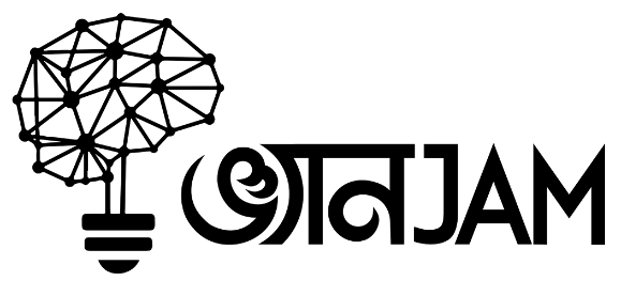
\includegraphics[scale=.4]{img/logo.png}\\[\bigskipamount]
}
\postauthor{\end{center}}
\title{Introduction to Machine Learning}
\date{}
\begin{document}
\maketitle
\section{Day 0}
Welcome to Machine Learning! Today you'll get yourself introduced with the idea of making a computer learn by itself without being explicitly programmed. You'll also see some classifications of Machine Learning problem, mainly:
\begin{itemize}
\item Supervised Learning
\begin{itemize}
\item Linear Regression
\item Logistic Regression
\item Linear Discriminant Analysis
\item K-Nearest Neighbors
\item Decision Trees
\end{itemize}
\item Unsupervised Learning
\begin{itemize}
\item K-Means Clustering
\item Principal Component Analysis
\item Anomaly Detection
\item Collaborative filtering and Recommender Systems
\end{itemize}
\item Reinfocement Learning
\end{itemize}
You can find the relevant materials for today in the links below:
\begin{itemize}
\item \href{https://www.youtube.com/watch?v=PPLop4L2eGk}{What Is Machine Learning}
\item \href{https://www.youtube.com/watch?v=bQI5uDxrFfA}{Supervised Learning}
\item \href{https://www.youtube.com/watch?v=jAA2g9ItoAc}{Unsupervised Learning}
\item \href{https://www.youtube.com/watch?v=JgvyzIkgxF0}{Reinforcement Learning}
\end{itemize}
\section{Day 1}
This day, you'll get to know the most widely used tools for Machine Learning that will speed up your Machine Learning algorithms with the help of cleverly optimized Linear Algebra libraries. This is possible because of a process called ``Vectorization'' which exploits the benefits of SIMD (Single Intruction Multiple Data) Parallelism, which speeds up your algorithms by a factor of ~ 400-600. Mainly, the tools that you'll be using through this course are:
\begin{itemize}
\item Python\\
There are some linear algebra libraries of python that you'll get accustomed to throughout this course.
\begin{itemize}
\item SciPy
\item NumPy
\item Matplotlib
\end{itemize}
\item JupyterLab
\item Conda
\item Examples of Data Visualization using Matplotlib
\item Basic Linear Algebra for Machine Learning
\end{itemize}
\begin{center}
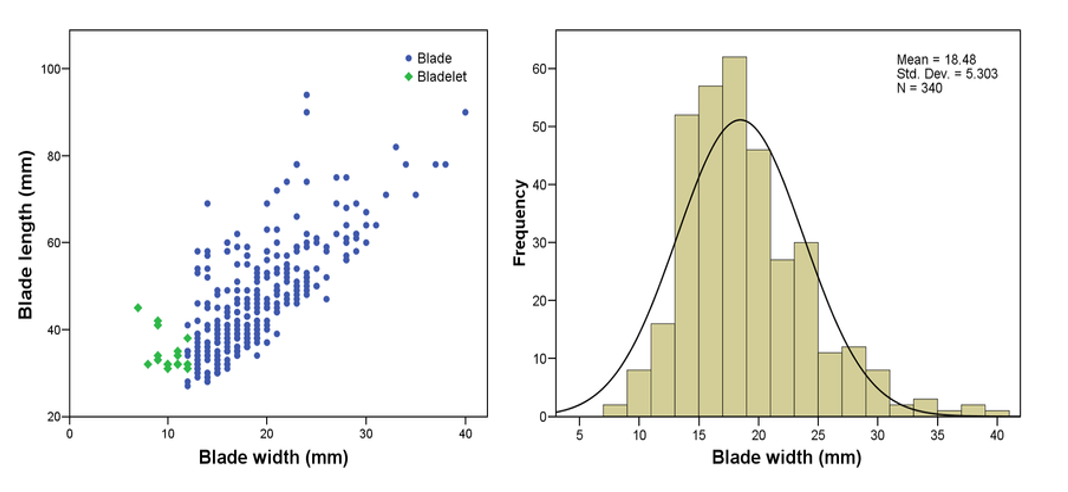
\includegraphics[scale=.7]{img/dataVis.png}
\end{center}
There are some links that you will need to visit frequently while exercising ML algorithms, and these are listed below for your convenience:
\begin{itemize}
\item \href{https://numpy.org/doc/stable/}{Numpy} Documentation
\item \href{https://matplotlib.org/contents.html}{Matplotlib} Documentation
\item \href{https://www.python.org/doc/}{Python} Documentation
\item \href{https://jupyterlab.readthedocs.io/en/stable/}{JupyterLab} Documentation
\item \href{https://www.youtube.com/watch?v=23aQdrS58e0}{Conda} Introduction
\end{itemize}
\pagebreak
\section{Day 2}
Today you will learn basic Linear Regression and Gradient Descent, as well as some optimization for your learning algorithms including Feature Scaling and Mean Normalization. You'll need to have a brief idea of basic differential calculus for Gradient Descent as a pre-requisite. Using Linear Regression and Gradient Descent, you can fit a linear model on a sample dataset as follows:\\
\begin{center}
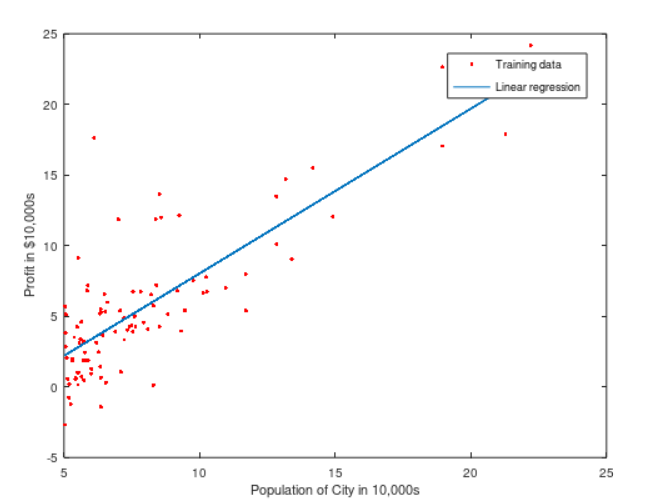
\includegraphics[scale=.7]{img/simplifiedGd.png}
\end{center}
List of relevant information and videos:
\begin{itemize}
\item \href{https://www.youtube.com/watch?v=kHwlB_j7Hkc}{Representing the model}
\item \href{https://www.youtube.com/watch?v=yuH4iRcggMw}{Squared error cost function}
\item \href{https://www.youtube.com/watch?v=e1nTgoDI_m8}{Feature scaling and Mean normalization}
\item \href{https://www.youtube.com/watch?v=YovTqTY-PYY}{Gradient Descent}
\end{itemize}
\pagebreak
\section{Day 3}
Logistic regression is a classification algorithm. Unlike regression algorithms which gives a continuous valued output, classification algorithms provide discrete valued output which can be used for creating decision boundaries and digit recognition.\\ 
\begin{center}
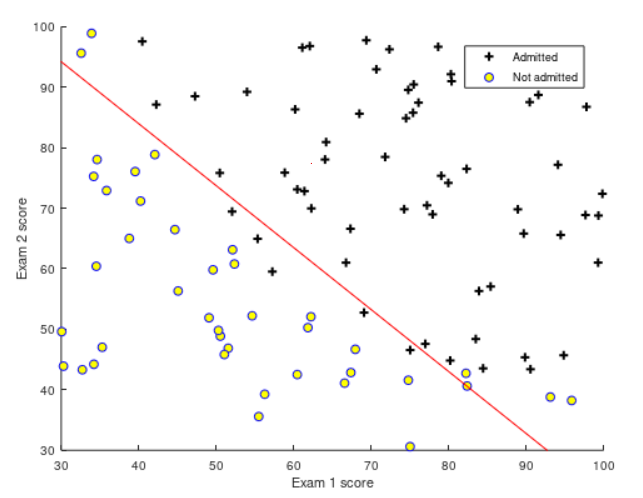
\includegraphics[scale=.7]{img/simplifiedLogReg}
\end{center}
Further optimizing the learning algorithms by using multiple features can be used to find out non-linear decision boundaries.
\begin{center}
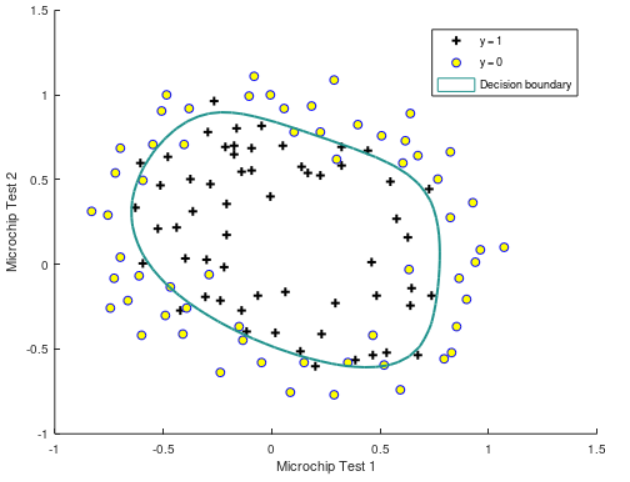
\includegraphics[scale=.7]{img/simplifiedRegLogReg.png}
\end{center}
\begin{itemize}
\item \href{https://www.youtube.com/watch?v=t1IT5hZfS48}{Logistic Regression concept}
\item \href{https://www.youtube.com/watch?v=F_VG4LNjZZ}{Decision boundary}
\item \href{https://www.youtube.com/watch?v=HIQlmHxI6-0}{Cost function for Logistic regression}
\item \href{https://www.youtube.com/watch?v=ISBGFY-gBug}{Bias and Variance}
\item \href{https://www.youtube.com/watch?v=KvtGD37Rm5I}{Regularization}
\end{itemize}
\section{Day 4}
More supervised learning algorithms will give you a brief overview of Linear Discriminant Analysis, K-Nearest Neighbors and Decision trees. 
\begin{figure}[h!]
\begin{center}
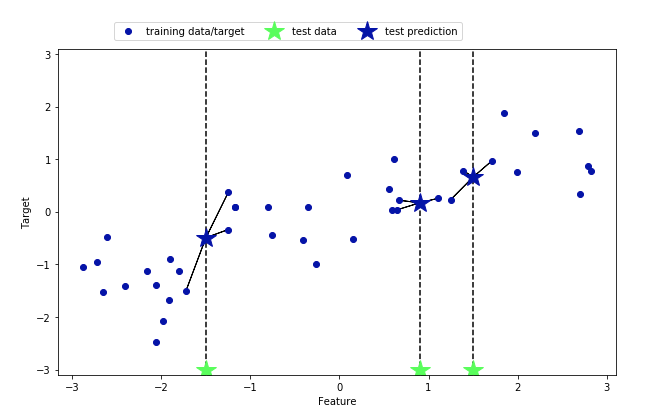
\includegraphics[scale=.5]{img/knn2.png}
\end{center}
{\caption*{K-Nearest Neighbors}}
\begin{center}
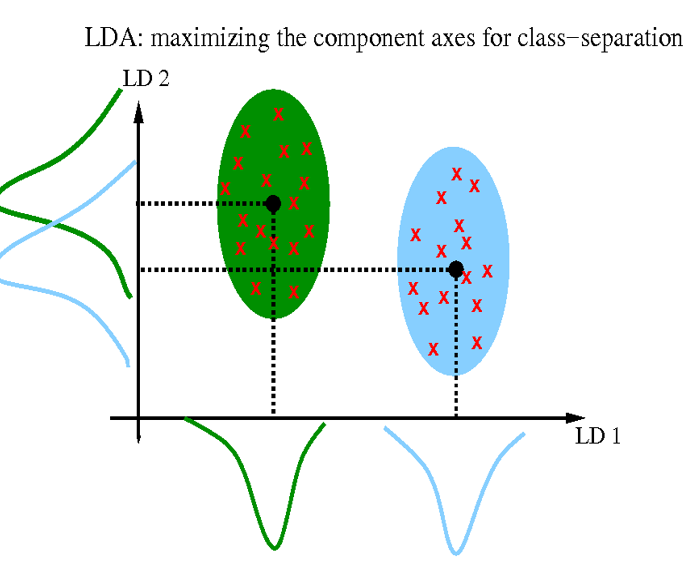
\includegraphics[scale=.6]{img/lda.png}
\end{center}
\end{figure}
\begin{itemize}
\item \href{https://www.youtube.com/watch?v=HVXime0nQeI}{K-Nearest Neighbors}
\item \href{https://www.youtube.com/watch?v=azXCzI57Yfc}{Linear Discriminant Analysis}
\item \href{https://www.youtube.com/watch?v=7VeUPuFGJHk}{Decision Trees}
\end{itemize}
\section{Day 5}
Measuring the performance of a learning algorithm is undoubtedly the most crucial part of a Machine Learning project. Using Matplotlib, learning curves can be plotted and be checked against overfitting or underfitting problems. Regularization can be addressed to tackle these issues. Exploiting the benefits of real-valued performance measurement and error metrics such as: Precision, Recall and F1 Score, we can further extract out the best result of our Machine Learning project by choosing the best parameters and learning algorithm.
\begin{figure}[h!]
\begin{center}
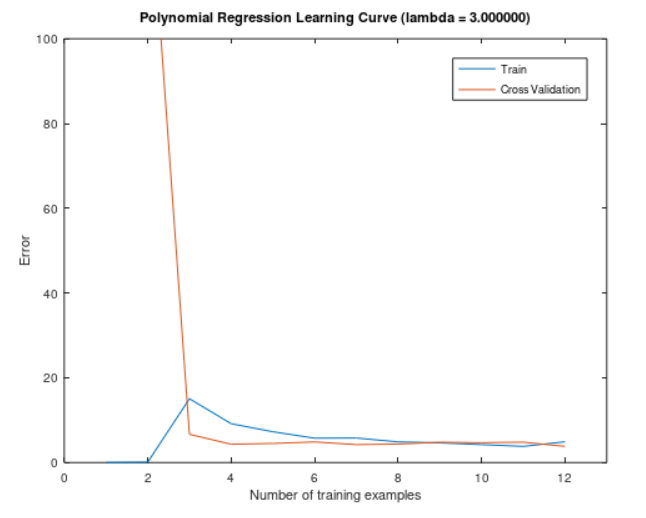
\includegraphics[scale=.8]{img/lc.png}
{\caption*{Learning Curve}}
\end{center}
\end{figure}\\
Useful links and materials:
\begin{itemize}
\item \href{https://www.youtube.com/watch?v=ISBGFY-gBug}{Learning Curves}
\item \href{https://www.youtube.com/watch?v=wGw6R8AbcuI}{Error Metrics}
\item \href{https://www.youtube.com/watch?v=W5meQnGACGo}{F1 Score}
\end{itemize}
\pagebreak
\section{Day 6}
Just using a logistic regression classifier to plot decision boundaries often fails to keep a large margin between the different classes, and this is where Large Margin Classifiers come into play. Support Vector Machines is undoubtedly one of the most widely used algorithm to address this issue. Using a suitable Kernel, a margin between different classes can be maintained in order to further improve the performance of your learning algorithms, and the best part is that you don't even have to implement any of these SVM algorithms by yourself. All these algorithms are neatly packed in your python libraries which you can apply using just a few lines of code!
\begin{figure}[h!]
\begin{center}
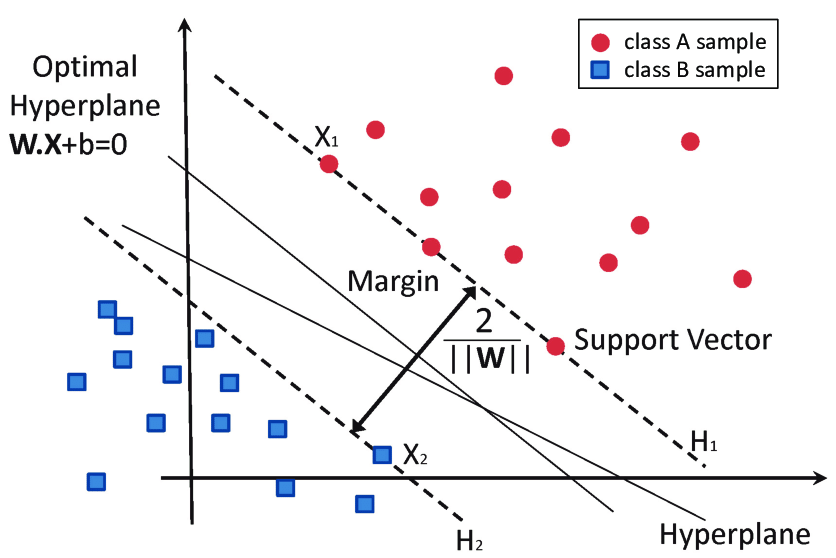
\includegraphics[scale=.45]{img/svm.png}
{\caption*{Support Vector Machine}}
\end{center}
\end{figure}\\
Useful links and materials:
\begin{itemize}
\item \href{https://www.youtube.com/watch?v=Ccje1EzrXBU}{Large Margin Intuition}
\item \href{https://www.youtube.com/watch?v=efR1C6CvhmE}{SVM explained}
\item \href{https://www.youtube.com/watch?v=mTyT-oHoivA}{Kernels}
\item \href{https://www.youtube.com/watch?v=7sz4WpkUIIs}{SVM with Python} [Warning: Long Video]
\end{itemize}
\pagebreak
\section{Day 7}
Unsupervised Learning Algorithms are used to find patterns/structures in a given dataset. The term `Unsupervised' is used because we don't have to use any labeled training examples as we had to in Supervised Algorithms. You will be able to analyze clusters in datasets by successfully implementing the very popular K-Means Clustering algorithm. You will also learn to compress an image from 24-bit to 16-bit representation by using the Principal Component Analysis algorithm, which will also help you with data compression.
\begin{figure}[h!]
\begin{center}
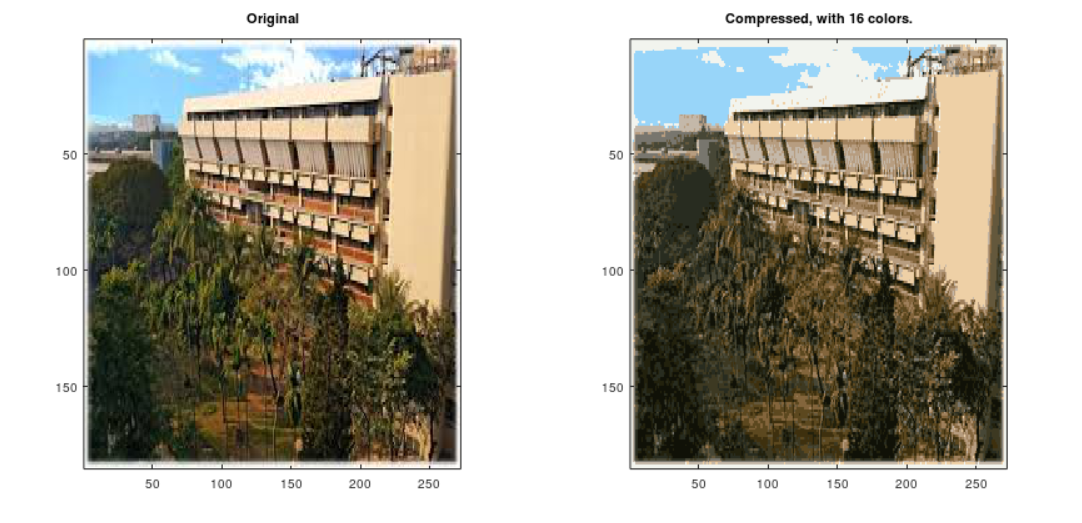
\includegraphics[scale=.6]{img/icKmC.png}
\end{center}
{\caption*{Image compression}}
    \centering
    \subfloat[Visualizing Dataset]{{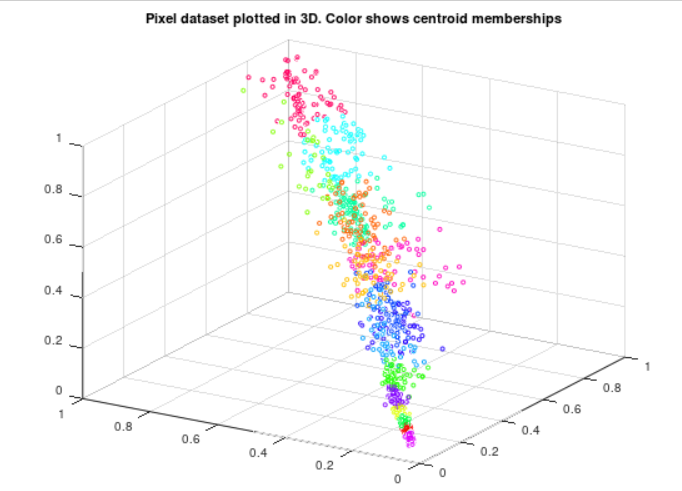
\includegraphics[scale=0.5]{img/pca1.png} }}%
    \qquad
    \subfloat[Reduced Dimension]{{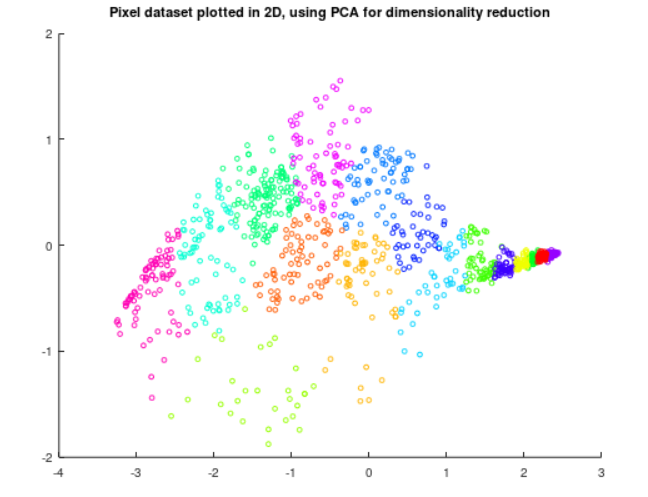
\includegraphics[scale=0.5]{img/pca2.png} }}%
    {\caption*{Principal Component Analysis}}%
    \label{fig:example}%
\end{figure}\\
Useful links and materials:
\begin{itemize}
\item \href{https://www.youtube.com/watch?v=hDmNF9JG3lo}{K-Means Clustering}
\item \href{https://www.youtube.com/watch?v=T-B8muDvzu0}{Principal Component Analysis-1}
\item \href{https://www.youtube.com/watch?v=rng04VJxUt4}{Principal Component Analysis-2}
\end{itemize}
\pagebreak
\section{Day 8}
You will learn how to detect anomalies in your system and this type of unsupervised learning is used in fraud detection, manufacturing aircraft engines, monitoring machines in data center and so on. Carefully chosen features will help your algorithms ouput the best prediction and using Gaussian Distribution, you can implement the Anomaly Detection algorithm by yourself.
\begin{figure}[h!]
\centering
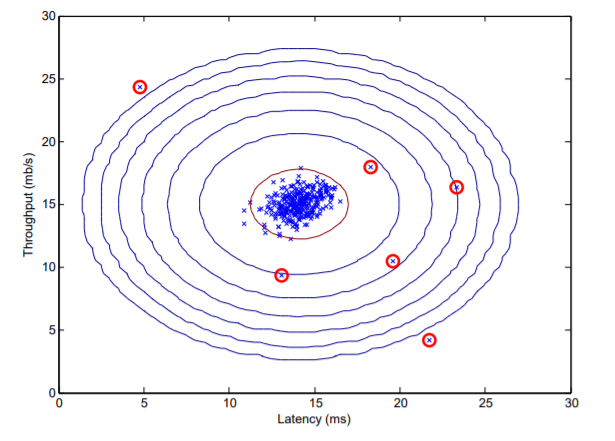
\includegraphics[scale=.8]{img/ad.png}
{\caption*{Anomaly Detection}}
\centering
\hspace*{-1.1cm}   
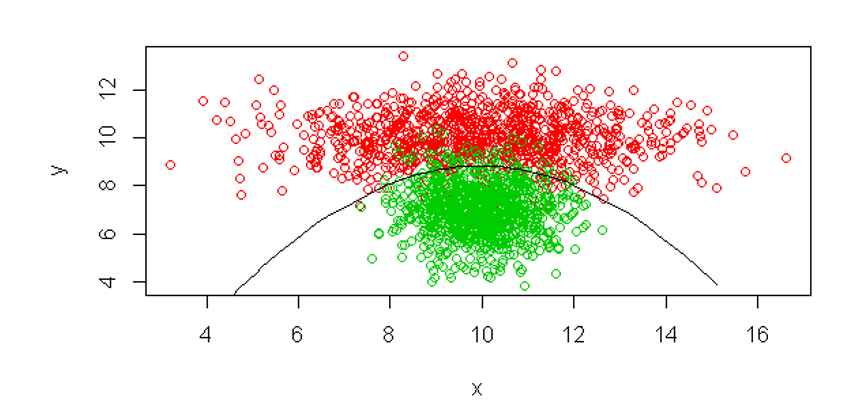
\includegraphics[scale=.6]{img/gnb.png}
{\caption*{Gaussian Naive Bayes}}
\end{figure}\\
Useful links and materials:
\begin{itemize}
\item \href{https://www.youtube.com/watch?v=mh6rAYA0e7Q}{Gaussian Distribution}
\item \href{https://www.youtube.com/watch?v=g2YBWQnqOpw}{Anomaly Detection algorithm}
\end{itemize}
\pagebreak
\section{Day 9}
Ever wondered how YouTube is able to accurately predict the videos that you are most likely to watch? Every time you watch a video, YouTube's Recommender System keeps track of your watch history. By analyzing your past videos, a recommender system can accurately predict what types of videos you will prefer and what types of videos you will not likely watch. The next time you go to YouTube, you will see your homepage flooded with recommendations, and most of those are bang on! These sorts of Recommender Systems work based on Collaborative Filtering and are widely used in online e-commerce services like Amazon, Daraz and Foodpanda, which contributes a substantial amount to their revenue.
\end{document}





















